\chapter{Approaches}
\label{ch:approaches}

The Thesis work follows the Deduction research approach where the theory is established based on own ideas in addition to literature review findings. \\ \\

The prototypes are created based on the established theory and user study is performed which follows Qualitative and Quantitative approaches in assimilating the results. It follows a well established Iterative process of UX Design cycle as seen in the following figure. \\ \\

Our approach leads an iterative process where initially prototypes with our novel ideas are evaluated by the target users. Next, the evaluation results lead to the requirements gathering phase. Then again, the prototypes are developed and so on the cycle repeats until the desired satisfaction of target users is achieved. \\ \\

In our Qualitative research methodology, the feedback of users is concerned as an example of emotional feeling on the usability of the designed prototype. On the other hand, in our Quantitative research methodology, we analyse some metrics on the results gathered during the evaluation phase. \\ \\

For every Research Question, the user scenario is formulated and what usual Static Code Analysis tool does. Next,  what can be done better considering other solution ideas from different Software Engineering domains in addition to our own ideas is analysed through the UX Design process. \\ \\

\begin{figure}[hbt!]
	\centering
	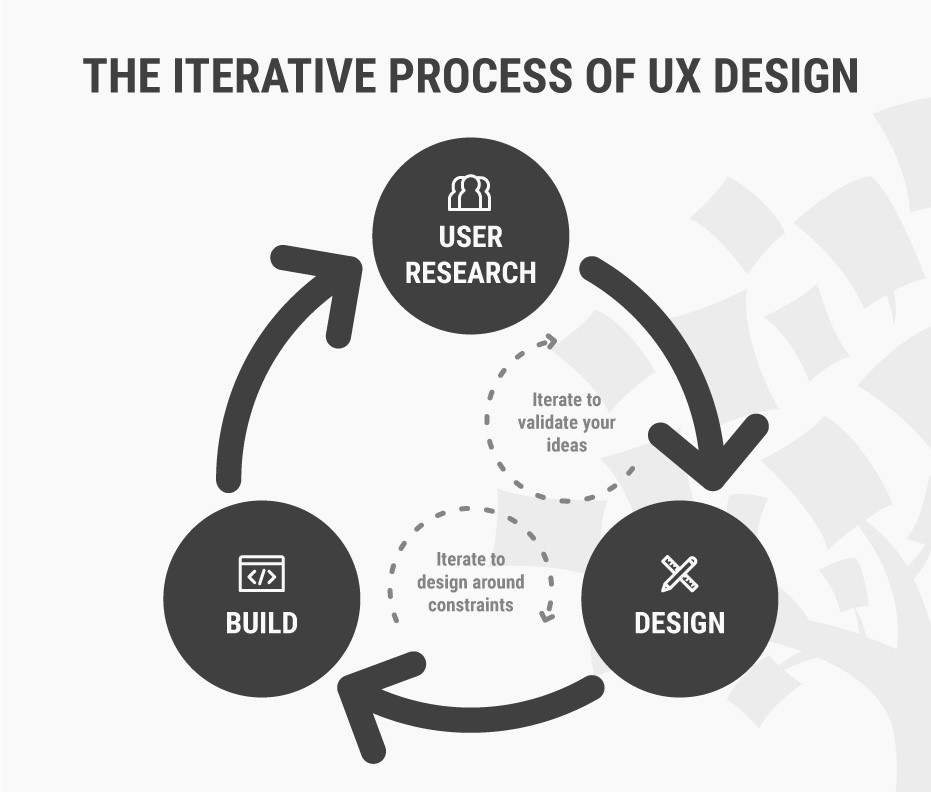
\includegraphics[width=\linewidth]{figures/ux-design}
	\caption{UX-Design.}
	\label{fig:ux-design}
\end{figure}